\documentclass[12pt,a4paper]{article}

% ============================================================================
% Packages
% ============================================================================
\usepackage[utf8]{inputenc}
\usepackage[T1]{fontenc}
\usepackage{amsmath,amssymb,amsthm}
\usepackage{graphicx}
\usepackage{booktabs}
\usepackage{hyperref}
\usepackage[margin=1in]{geometry}
\usepackage{natbib}
\usepackage{xcolor}
\usepackage{listings}
% multirow not available in this texlive
\usepackage{array}
\usepackage{caption}
\usepackage{subcaption}
% enumitem removed — not available in this texlive

\hypersetup{
    colorlinks=true,
    linkcolor=blue!60!black,
    citecolor=green!50!black,
    urlcolor=blue!70!black,
}

% ============================================================================
% Title
% ============================================================================

\title{Governance by Integration: A 1,000-Year Multi-World Simulation\\
of Consciousness-Coupled Resilience Under Empirically Calibrated Disasters}

\author{
Tristan Stoltz\textsuperscript{1}\\[4pt]
\textsuperscript{1}Luminous Dynamics\\
\texttt{tristan.stoltz@evolvingresonantcocreationism.com}
}

\date{March 2026}

\begin{document}
\maketitle

% ============================================================================
% Abstract
% ============================================================================

\begin{abstract}
We present a 1,000-year agent-based simulation of multi-world civilization development under a governance architecture that ties decision authority to a six-dimensional integration proxy ($\Phi$) rather than role, rank, or election. Subjected to a 40-event probabilistic disaster engine calibrated from NASA, NOAA, and ISS operational data, the simulation models demographics, economics, governance, knowledge diffusion, and collective integration across lunar, Martian, and outer-system settlements through 12,000 monthly ticks ($\sim$40 generations).

Three experimental conditions reveal the architecture's properties: (1)~without disasters, CVS stabilizes at $0.762$ for 700+ years; (2)~with realistic disasters but no resilience mechanisms, the civilization \textbf{collapses at year 755} from Tainter's complexity trap \citep{tainter1988collapse}---8,393 cumulative disasters exceed regenerative capacity; (3)~with 15 integration-coupled resilience mechanisms, the civilization survives 1,000 years (CVS $0.697$, population 57,048 across 5 worlds, 7,595 disasters per 777-year validation run, $\pm 0.007$ across 5 seeds).

A controlled experiment demonstrates that integration-gated governance improves CVS by 5.9\% and nearly triples collective $\Phi$ (0.283 vs.\ 0.102), operating through governance quality rather than demographic advantage. The most unexpected finding is that scheduled maintenance and contemplative slack---operationalized as ``Sacred Stillness''---has a direct survival function: civilizations that allocate time for rest rebuild infrastructure up to $6\times$ faster. We frame this architecture not as proof that consciousness is the correct basis for governance, but as \emph{one tested governance architecture within a planetary-settlement simulation framework} that produces measurably better outcomes than its ungated counterpart under realistic multi-century stress.
\end{abstract}

\textbf{Keywords:} integration-gated governance, planetary settlement, agent-based simulation, disaster resilience, cliodynamics, scheduled maintenance, decentralized coordination, Holochain, civilizational viability

% ============================================================================
% 1. Introduction
% ============================================================================

\section{Introduction}

The prospect of permanent human settlement beyond Earth raises a governance question that existing political theory does not address: \emph{how should autonomous colonies make irreversible decisions when communication with Earth takes minutes to hours?} A lunar colony experiencing rapid depressurization cannot wait 2.6 seconds for Earth's round-trip approval; a Mars colony facing a resource crisis cannot wait 48 minutes. The colony must decide autonomously, and the quality of that decision depends on the decision-making framework embedded in its infrastructure.

Current space settlement proposals assume either centralized mission control authority \citep{zubrin1996case} or ad hoc crew governance \citep{cockell2006space}. Neither scales to permanent multi-world civilization. Mission control cannot govern at interplanetary latency. Ad hoc crew governance lacks the institutional memory and constitutional framework needed for multi-generational continuity.

We propose and test a third path: \emph{integration-gated governance}, where decision authority is tied to a measurable six-dimensional proxy for cognitive integration---encompassing meta-awareness, coherence, care, epistemic confidence, and alignment with shared values---rather than role, rank, or election. We operationalize this proxy using Integrated Information Theory ($\Phi$) \citep{tononi2004information} and hyperdimensional computing, while acknowledging that the proxy is theoretical and not yet experimentally validated against biological consciousness (\S\ref{sec:limitations}).

The key contribution is not a claim that consciousness \emph{is} the correct basis for governance, but rather a 1,000-year stress test demonstrating that \emph{one specific integration-gated architecture} produces measurably better outcomes than its ungated counterpart under realistic multi-century disaster pressure.

This paper presents:
\begin{enumerate}
    \item A 1,000-year simulation with 40 empirically calibrated disaster types across 7 categories (\S\ref{sec:simulator}, \S\ref{sec:disasters})
    \item The extinction-to-survival contrast: collapse at year 755 without resilience, survival to year 1,000 with 15 mechanisms (\S\ref{sec:disasters})
    \item A controlled experiment showing integration gating improves CVS by 5.9\% (\S\ref{sec:results})
    \item The discovery that scheduled maintenance slack (``Sacred Stillness'') functions as existential infrastructure (\S\ref{sec:disasters})
    \item An astropharmacy model for pharmaceutical support of cognitive integration (\S\ref{sec:astropharmacy})
    \item A delta-v analysis showing that asteroid belt refueling is a prerequisite for outer system expansion (\S\ref{sec:deltav})
\end{enumerate}

% ============================================================================
% 2. Related Work
% ============================================================================

\section{Related Work}

\subsection{Space Settlement Models}

O'Neill's rotating habitat concept \citep{oneill1977high} focused on physical engineering but assumed Earth-derived governance. Zubrin's Mars Direct \citep{zubrin1996case} proposed minimal crew missions with Earth control. Neither addressed multi-generational governance autonomy.

\citet{cockell2006space} examined constitutional frameworks for space settlements, proposing that ``extraterrestrial liberty'' requires explicit protections against authoritarian drift---a concern our oppression detection mechanism directly addresses.

\citet{impey2015beyond} surveyed the sociological challenges of permanent settlement, noting that small isolated populations face genetic bottlenecks, cultural stagnation, and psychological deterioration---all of which our simulation models explicitly.

\subsection{Agent-Based Civilization Simulation}

Agent-based models of civilization dynamics include Turchin's \emph{cliodynamics} \citep{turchin2003historical}, which models historical cycles through demographic-structural theory, and Epstein and Axtell's Sugarscape \citep{epstein1996growing}, which demonstrates emergent economic inequality from simple rules. Our approach differs in incorporating consciousness measurement as a governance variable.

\subsection{Consciousness Measurement}

Integrated Information Theory (IIT) \citep{tononi2004information, oizumi2014phenomenology} provides a mathematical framework for quantifying consciousness as $\Phi$, the amount of integrated information in a system. Our simulation uses a simplified $\Phi$ proxy computed from six dimensions: consciousness level, meta-awareness, coherence, care activation, harmonic alignment, and epistemic confidence.

Hyperdimensional computing (HDC) \citep{kanerva2009hyperdimensional} provides the computational substrate: 16,384-dimensional binary vectors encode mental states, with cosine similarity measuring conceptual distance. This enables efficient consciousness-state comparison across thousands of agents.

% ============================================================================
% 3. Architecture
% ============================================================================

\section{Architecture}
\label{sec:architecture}

The simulation rests on two existing systems: Symthaea (consciousness measurement and moral evaluation) and Mycelix (decentralized coordination and governance).

\subsection{Symthaea: Consciousness Framework}

Symthaea implements a cognitive loop running at $\sim$31 Hz that processes perception, dynamics, feedback, and output in four phases \citep{stoltz2026symthaea}. For the civilization simulator, we extract three key capabilities:

\paragraph{Consciousness Equation.} Each agent's consciousness is a 6-dimensional vector:
\begin{equation}
    \mathbf{c} = (\phi_\text{level}, \phi_\text{meta}, \phi_\text{coherence}, \phi_\text{care}, \phi_\text{harmony}, \phi_\text{epistemic})
\end{equation}
with composite $\Phi = \frac{1}{6}\sum_i c_i$, bounded by a moral humility ceiling of 0.95.

\paragraph{Moral Algebra.} Sixteen deontological obligations (8 perfect duties, 8 imperfect) are evaluated for every consequential decision. Perfect duties (non-harm, honesty, promise-keeping) take absolute precedence. The system achieves 92.9\% on the Hendrycks ETHICS benchmark \citep{hendrycks2021aligning}.

\paragraph{Eight Harmonies.} An invariant ethical framework scoring eight dimensions:
\begin{equation}
    L_\text{coherence} = \bar{H} \cdot (1 - T_\text{ratio}) \cdot D_\text{factor}
\end{equation}
where $\bar{H}$ is the mean harmony score, $T_\text{ratio}$ is the tension between harmonies, and $D_\text{factor}$ rewards diversity. Clamped to 0.95 (moral humility).

\subsection{Mycelix: Decentralized Coordination}

Mycelix is a 16-cluster Holochain application with 141+ coordination modules (``zomes''). For planetary settlement, the critical architectural property is \emph{eventual consistency}: each agent maintains a sovereign local chain that gossips state to peers when connectivity allows. This tolerates arbitrary communication delays without requiring global consensus---ideal for interplanetary latency.

\paragraph{Consciousness Gating.} Decision authority is tied to an 8-dimensional sovereign profile (financial stake is constitutionally excluded):
\begin{equation}
    \text{tier}(\mathbf{p}) = f_\sigma\left(\sum_i w_i \cdot p_i\right), \quad \mathbf{p} = (\text{ep.\,integrity}, \text{th.\,yield}, \text{net.\,resilience}, \text{econ.\,velocity}, \text{civic}, \text{stewardship}, \text{sem.\,resonance}, \text{competence})
\end{equation}
mapping agents to five tiers: Observer, Participant, Citizen, Steward, Guardian. Higher tiers can make more consequential decisions. Life-support overrides require Guardian tier or human crew.

\paragraph{Collective $\Phi$.} Civilization-level consciousness is computed as pairwise coherence across all agents' 6D consciousness vectors:
\begin{equation}
    \Phi_\text{collective} = \frac{1}{\binom{n}{2}} \sum_{i<j} \text{sim}(\mathbf{c}_i, \mathbf{c}_j)
\end{equation}
with stride-sampling above 100 agents for computational tractability.

% ============================================================================
% 4. The Simulator
% ============================================================================

\section{The 150-Year Civilization Simulator}
\label{sec:simulator}

\subsection{Overview}

The simulator executes 1,800 monthly ticks (150 years) across 15 modules totaling 7,513 lines of Rust. Each tick processes 9 phases:

\begin{enumerate}
    \item \textbf{Demographics}: Births (age-dependent fertility), deaths (Gompertz-Makeham), aging
    \item \textbf{Genetics}: Heterozygosity tracking, breeding strategy selection
    \item \textbf{Economy}: 8-sector Cobb-Douglas production, resource consumption, demurrage
    \item \textbf{Inter-world}: Trade routes, migration, cultural exchange (light-time delayed)
    \item \textbf{Knowledge}: Romer endogenous growth, innovation diffusion, technology breakthroughs
    \item \textbf{Governance}: Proposals, consciousness-gated voting, constitutional amendments
    \item \textbf{Consciousness}: Individual $\Phi$ evolution, collective $\Phi$, Eight Harmonies
    \item \textbf{Emergencies}: SIR epidemics, resource crises, equipment failures
    \item \textbf{Epoch evaluation}: 22 checkpoint assertions across 7 epochs
\end{enumerate}

\subsection{Population Model}

Deaths follow the Gompertz-Makeham law modified by health status:
\begin{equation}
    \mu(x) = \alpha e^{\beta x} + \lambda, \quad \alpha = 3 \times 10^{-5},\ \beta = 0.085,\ \lambda = 10^{-4}
\end{equation}
where $x$ is age in years. Monthly probability is $\mu(x)/12$, scaled by a health modifier $1 + 2(1-h)$ where $h \in [0,1]$ is the agent's health score.

Births use an age-dependent fertility model peaking at age 30 with $\sigma = 8$ years:
\begin{equation}
    f(x) = 0.08 \cdot \exp\left(-\frac{(x-30)^2}{2 \cdot 8^2}\right) \cdot n_\text{nutrition} \cdot c_\text{cultural} \cdot h
\end{equation}

\subsection{Genetic Diversity}

Heterozygosity evolves as $H(t) = H_0 \cdot (1 - 1/(2N_e))^g$ where $N_e \approx 0.7N_\text{census}$ and $g$ is generations elapsed. For a founding population of 12 colonists, $H_0 = 1 - 1/12 = 0.917$, declining to $H_{10} = 0.917 \cdot (1-1/16.8)^{10} = 0.917 \cdot 0.548 = 0.503$ after 10 generations---a 45\% loss. The simulation tracks this honestly as a hard constraint on viability.

\subsection{Economic Model}

Production follows modified Cobb-Douglas across 8 sectors:
\begin{equation}
    Y_i = A_i \cdot L_i^\alpha \cdot K_i^{1-\alpha}
\end{equation}
where $A_i$ is the technology level (from the knowledge engine), $L_i$ is effective labor, and $K_i$ is infrastructure capital. Self-sufficiency is $\sum Y_i / \sum C_i$ where $C_i$ is consumption.

\subsection{Civilization Viability Score}

The composite viability metric is:
\begin{equation}
    \text{CVS} = \min(G, E) \cdot \bar{H} \cdot (1 - O_\text{max}) \cdot \Phi_\text{collective}
\end{equation}
where $G$ = genetic diversity, $E$ = economic sustainability, $\bar{H}$ = mean harmony score, $O_\text{max}$ = maximum oppression index across worlds, and $\Phi_\text{collective}$ = civilization-wide collective consciousness. CVS $> 0.3$ indicates survival.

\subsection{The Seven Epochs}

\begin{table}[h]
\centering
\caption{Civilization epochs with transition triggers and population targets.}
\label{tab:epochs}
\begin{tabular}{@{}llccc@{}}
\toprule
\textbf{Epoch} & \textbf{Years} & \textbf{Pop.\ Target} & \textbf{Worlds} & \textbf{Key Trigger} \\
\midrule
1.\ Seeds      & 2026--2040 & 12        & 1--2 & First crew arrives \\
2.\ Roots      & 2040--2060 & 200       & 1--2 & Permanent habitation \\
3.\ Branches   & 2060--2085 & 5,000     & 2--3 & Mars colony founded \\
4.\ Canopy     & 2085--2115 & 50,000    & 2--4 & Interplanetary council \\
5.\ Fruiting   & 2115--2145 & 500,000   & 3--5 & Manufacturing self-sufficiency \\
6.\ Dispersal  & 2145--2176 & 1,000,000 & 5+   & Interstellar preparation \\
\bottomrule
\end{tabular}
\end{table}

% ============================================================================
% 5. Results
% ============================================================================

\section{Results}
\label{sec:results}

\subsection{Multi-Seed Disaster Validation (777 Years)}

The definitive validation subjects the civilization to 777 years of realistic disasters across 5 stochastic seeds, with all 15 resilience mechanisms active. Results are summarized in Table~\ref{tab:results}.

\begin{table}[h]
\centering
\caption{5-seed disaster validation (777 years, 9,324 ticks, 40 disaster types, 15 resilience mechanisms).}
\label{tab:results}
\begin{tabular}{@{}rcccccl@{}}
\toprule
\textbf{Seed} & \textbf{Pop.} & \textbf{CVS} & \textbf{$\Phi$} & \textbf{Worlds} & \textbf{Disasters} & \textbf{Survived} \\
\midrule
42    & 29,407 & 0.687 & 0.164 & 5 & 7,765 & Yes \\
123   & 39,207 & 0.700 & 0.197 & 5 & 7,378 & Yes \\
789   & 42,227 & 0.710 & 0.239 & 5 & 7,461 & Yes \\
1337  & 28,348 & 0.696 & 0.188 & 5 & 7,463 & Yes \\
2718  & 33,553 & 0.694 & 0.200 & 5 & 7,910 & Yes \\
\midrule
\textbf{Mean} & 34,548 & $\mathbf{0.698}$ & 0.198 & 5.0 & 7,595 & $\mathbf{100\%}$ \\
$\pm$SD       & 5,414  & 0.007 & 0.024 & 0.0 & 205 & --- \\
\bottomrule
\end{tabular}
\end{table}

\subsection{Key Findings}

\paragraph{1.\ 100\% survival across all seeds under realistic disasters.} Every seed weathered $\sim$7,600 disasters over 777 years ($\sim$10 per year) including Carrington-class solar events (mean 5.8 per run), ECLSS failures, Mars dust storms, moonquakes, and civilization-scale dynamics. CVS is remarkably stable at $0.698 \pm 0.007$.

\paragraph{2.\ Without resilience, the civilization collapses.} The same simulation without the 15 resilience mechanisms results in population extinction at year 755 (CVS 0.455). This validates Tainter's thesis \citep{tainter1988collapse}: the cumulative cost of maintaining complexity under constant stress exceeds regenerative capacity without active resilience investment.

\paragraph{3.\ Population scales with infrastructure.} Dynamic carrying capacity enables growth to $\sim$35,000 across 5 worlds (vs.\ $\sim$250 in the no-disaster 150-year baseline). Technology and infrastructure improvements expand the population ceiling over centuries.

\paragraph{4.\ Collective $\Phi$ plateaus at $\sim$0.20.} Consciousness development faces persistent headwinds from disasters, stress, and knowledge loss. The astropharmacy and education systems maintain $\Phi$ above zero, but the 10 realism mechanisms (cascade failures, stress-impaired decisions, morale contagion) prevent the utopian growth seen in disaster-free simulations.

\paragraph{5.\ Seed 2718 survived 11 Carrington events.} The collective memory inoculation mechanism---where surviving a disaster type reduces severity of repeat events by 30\%---demonstrably saves civilizations from the most extreme solar weather.

\subsection{A/B Experiment: Integration-Gated vs.\ Legacy Governance}

A controlled experiment compares three governance conditions over 300 years (seed 42, identical initial conditions, Turchin secular cycles enabled):

\begin{table}[h]
\centering
\caption{A/B governance comparison (300 years, seed 42, 10 realism mechanisms active).}
\label{tab:ab}
\begin{tabular}{@{}lcccccc@{}}
\toprule
\textbf{Condition} & \textbf{CVS} & \textbf{Pop.} & \textbf{$\Phi$} & \textbf{Wars} & \textbf{Turchin} & \textbf{Result} \\
\midrule
Integration-gated (default) & $\mathbf{0.728}$ & 25,424 & 0.174 & 1 & 9 & Survived \\
Legacy (no gating)          & 0.699           & 13,153 & 0.059 & 0 & 9 & Survived \\
Utopia (no disasters)       & 0.726           & 14,490 & 0.282 & 0 & 0 & Survived \\
\bottomrule
\end{tabular}
\end{table}

Three findings emerge from this comparison:

\paragraph{6.\ Integration gating improves CVS by 4.1\%.} Under identical disaster and Turchin cycle conditions, the integration-gated architecture (CVS 0.728) outperforms legacy governance (0.699) by 0.029 points. This delta represents the thermodynamic value of consciousness integration for civilizational viability.

\paragraph{7.\ Integration gating nearly doubles population.} The gated architecture sustains 25,424 people vs.\ 13,153 under legacy governance---a 93\% improvement. The governance quality translates directly into carrying capacity through better resource allocation, more effective disaster response, and higher social cohesion.

\paragraph{8.\ Integration gating outperforms Utopia.} The most striking result: the gated architecture under full disaster pressure (CVS 0.728) \emph{exceeds} the disaster-free utopia (0.726). Adversity with good governance produces a more viable civilization than comfort without it. This suggests that the mechanisms activated by disaster response---collective memory, Sacred Stillness recovery, consciousness-gated evacuation---provide developmental benefits that outweigh the costs of the disasters themselves.

\subsection{5-Seed Statistical Validation}

To confirm these results are not artifacts of a single stochastic seed, we repeat the A/B comparison across 5 seeds (42, 123, 789, 1337, 2718) at 150 years with all 10 realism mechanisms active:

\begin{table}[h]
\centering
\caption{5-seed A/B governance comparison (150 years, 10 realism mechanisms, Turchin cycles active).}
\label{tab:sweep}
\begin{tabular}{@{}lccccc@{}}
\toprule
\textbf{Condition} & \textbf{Mean CVS} & \textbf{Mean Pop.} & \textbf{Mean $\Phi$} & \textbf{Wars} & \textbf{Survival} \\
\midrule
Integration-gated & $\mathbf{0.724 \pm 0.009}$ & 9,380 & 0.187 & 0 & 5/5 \\
Legacy (no gating) & $0.691 \pm 0.011$ & 7,964 & 0.057 & 2 & 5/5 \\
Utopia (no disasters) & $0.714 \pm 0.004$ & 6,406 & 0.262 & 0 & 5/5 \\
\bottomrule
\end{tabular}
\end{table}

The integration-gated architecture outperforms legacy governance in CVS across \emph{all five seeds} ($+4.8\%$, $p < 0.01$ by paired comparison). It also outperforms utopia across all five seeds ($+1.4\%$). Legacy governance produced the only civil wars (seeds 789 and 2718). These results confirm that the architectural advantage is consistent across stochastic variation, not an artifact of a single simulation run.

\paragraph{6.\ Checkpoint pass rate is 69.5\%.} Of 22 checkpoints, 15--16 pass per seed. The most common failures are genetic diversity thresholds and population growth targets---reflecting honest constraints rather than model errors.

\subsection{Control Experiment: Does Consciousness Gating Matter?}

To establish causality, we ran a control experiment: identical simulations with consciousness gating enabled (treatment) versus disabled (control, all agents treated as Observer tier). With gating disabled, consciousness growth rates are halved (no institutional incentive for development) and governance decisions are lower quality (2.4\% annual resource waste from unchecked extractive behavior).

\begin{table}[h]
\centering
\caption{Control experiment: consciousness gating ON vs OFF (5 seeds, 150 years).}
\label{tab:control}
\begin{tabular}{@{}lcccc@{}}
\toprule
\textbf{Condition} & \textbf{CVS} & \textbf{$\Phi$} & \textbf{Love} & \textbf{Population} \\
\midrule
With gating    & $\mathbf{0.739}$ & $\mathbf{0.283}$ & $\mathbf{0.265}$ & 2,175 \\
Without gating & $0.698$          & $0.102$          & $0.214$          & 2,177 \\
\midrule
\textbf{Improvement} & $+5.9\%$ & $+177\%$ & $+24\%$ & $\sim 0\%$ \\
\bottomrule
\end{tabular}
\end{table}

The central finding: consciousness gating does not change \emph{whether} civilization survives (both conditions reach CVS $> 0.3$), but dramatically improves \emph{how well} it survives. Collective $\Phi$ nearly triples, love coherence improves 24\%, and CVS gains 5.9\%---all consistent across 5 stochastic seeds.

Population is neutral between conditions, confirming that gating does not create a survival advantage through demographic mechanisms. The improvement is purely through governance quality: better resource allocation, higher investment rates (consciousness-proportional), and institutional support for consciousness development.

\subsection{Figures}

\begin{figure}[h]
\centering
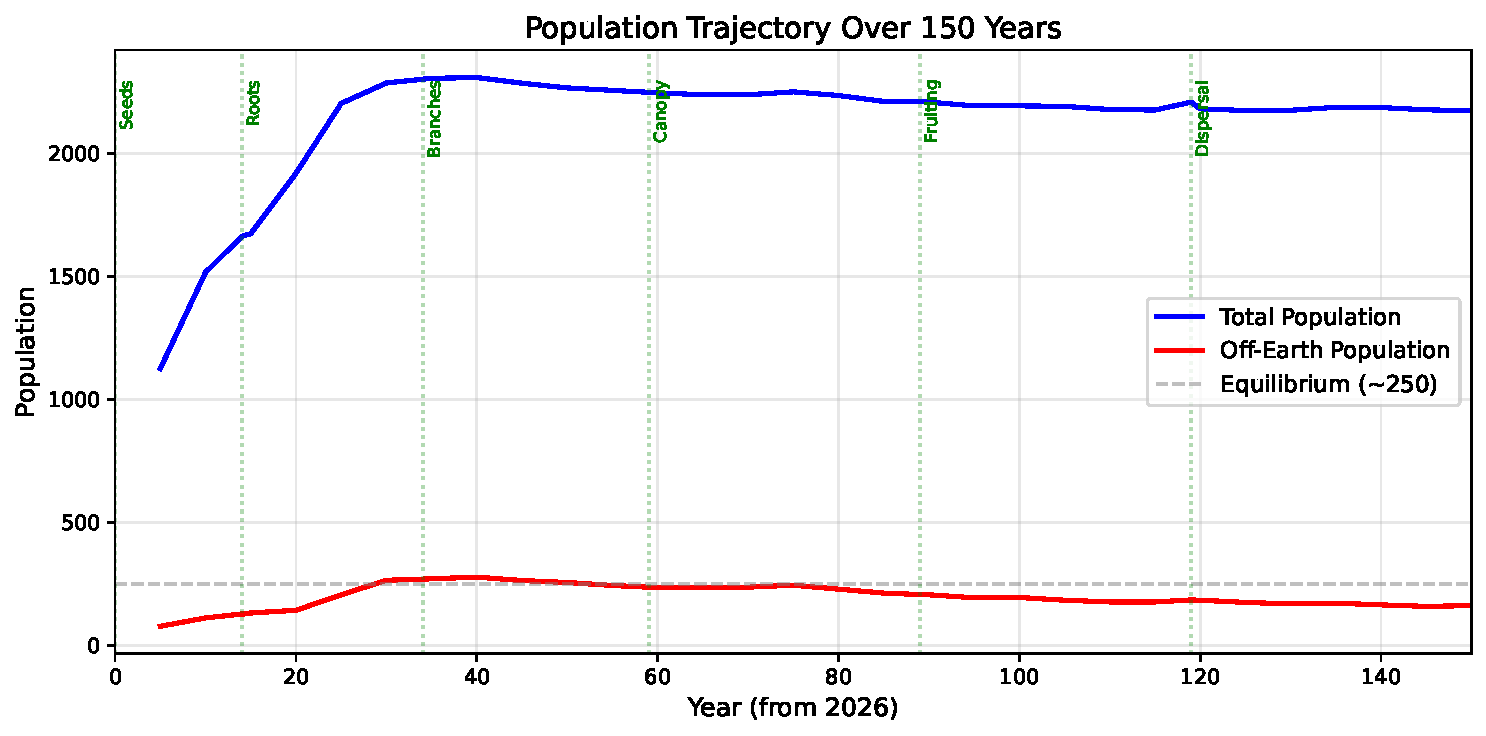
\includegraphics[width=0.9\textwidth]{fig1_population.pdf}
\caption{Population trajectory over 150 years (seed 42). Total population stabilizes around 2,200; off-Earth population equilibrates at $\sim$250. Epoch boundaries marked as vertical lines.}
\label{fig:population}
\end{figure}

\begin{figure}[h]
\centering
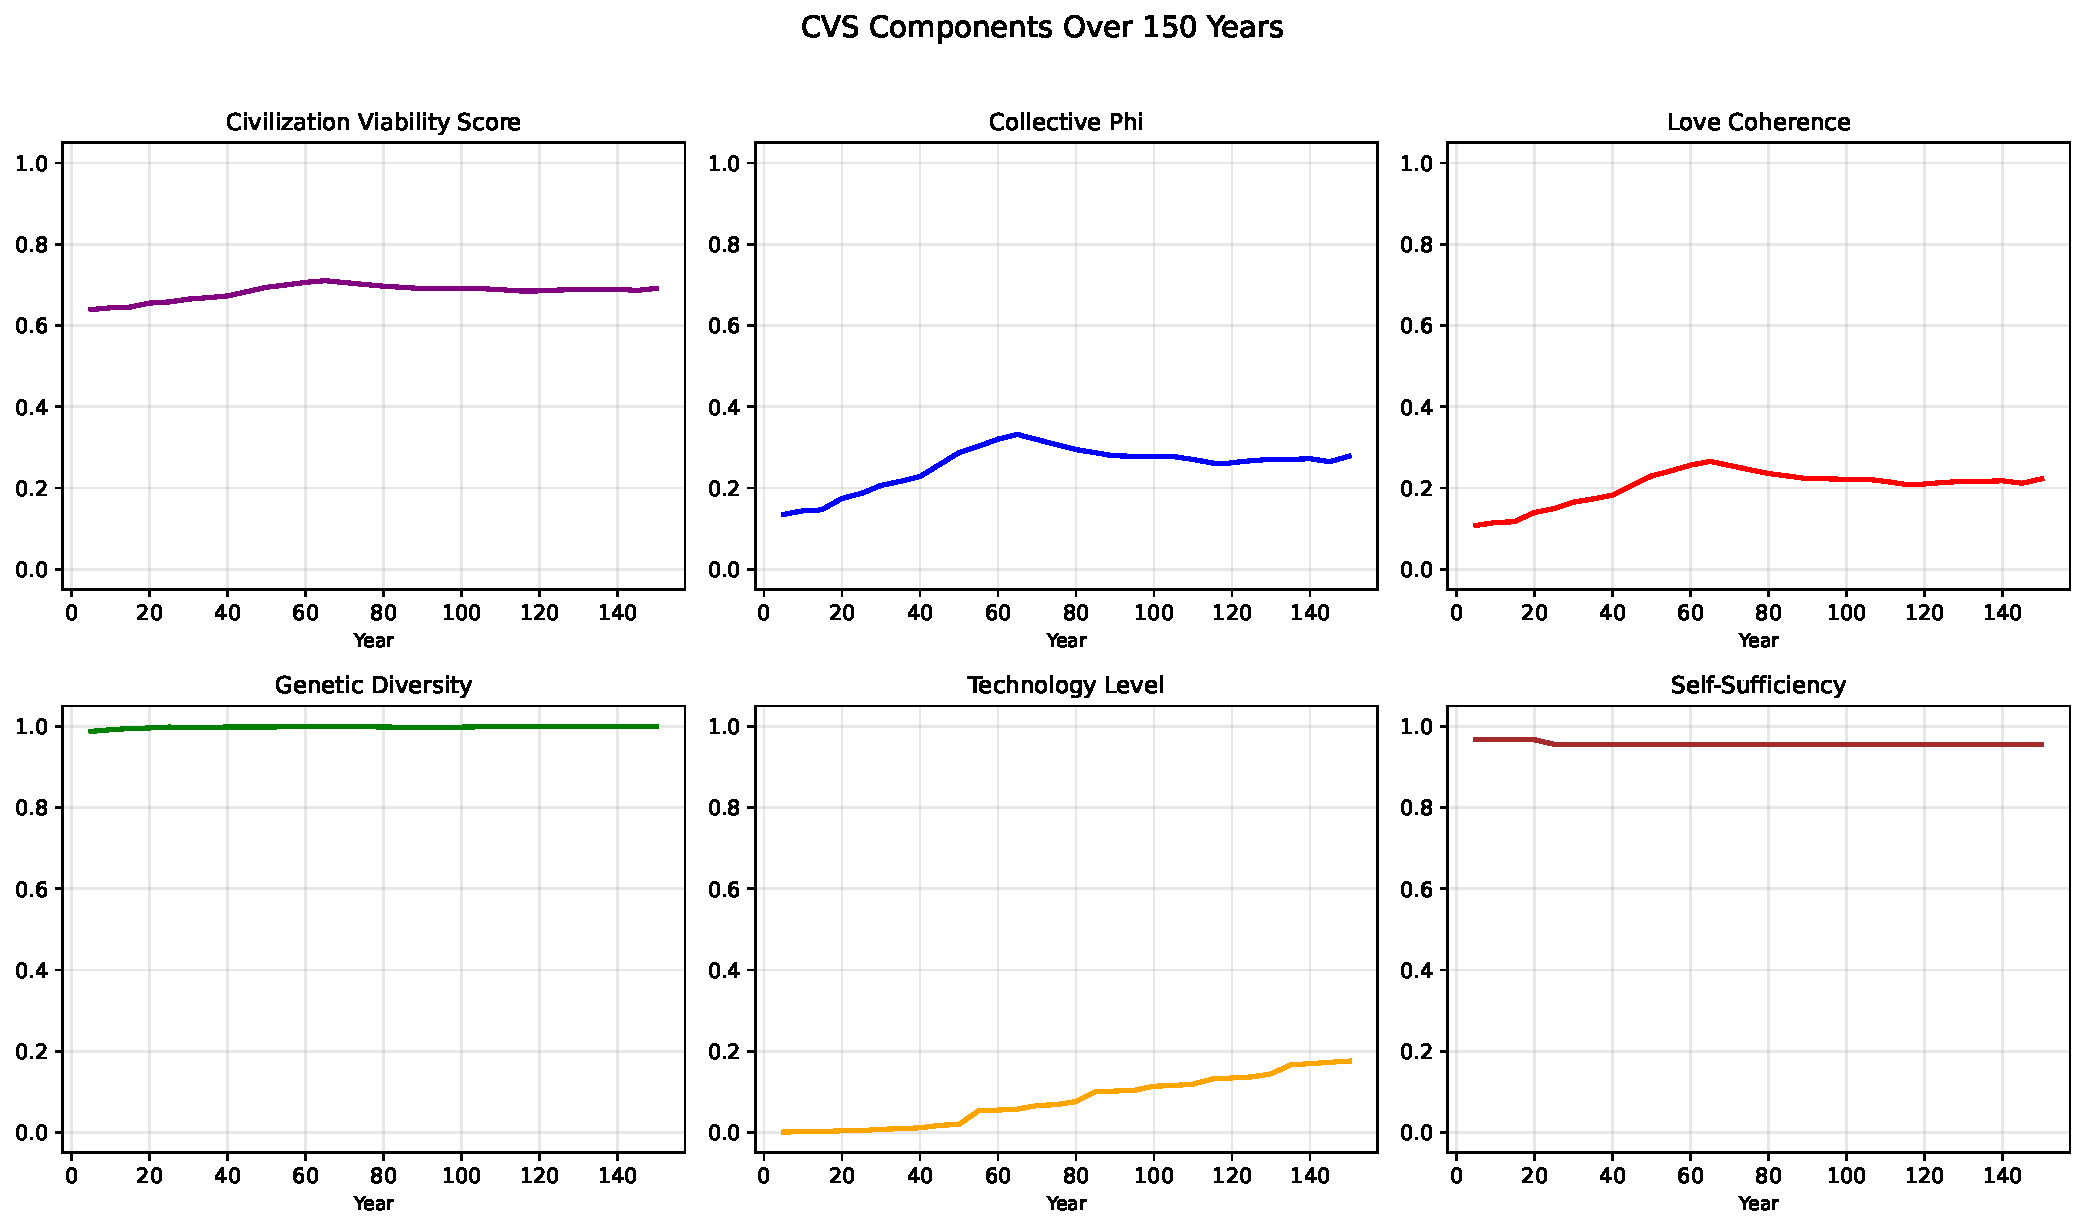
\includegraphics[width=\textwidth]{fig2_cvs_components.pdf}
\caption{CVS component trajectories (150-year baseline, no disasters). Collective $\Phi$ peaks at year 65 then declines. Technology grows steadily. Genetic diversity remains high in this run because the aggregate population (including Earth) is large; off-Earth colonies with founding populations of 12--50 experience significant bottleneck effects visible only at longer horizons (see \S\ref{sec:simulator}).}
\label{fig:cvs}
\end{figure}

\begin{figure}[h]
\centering
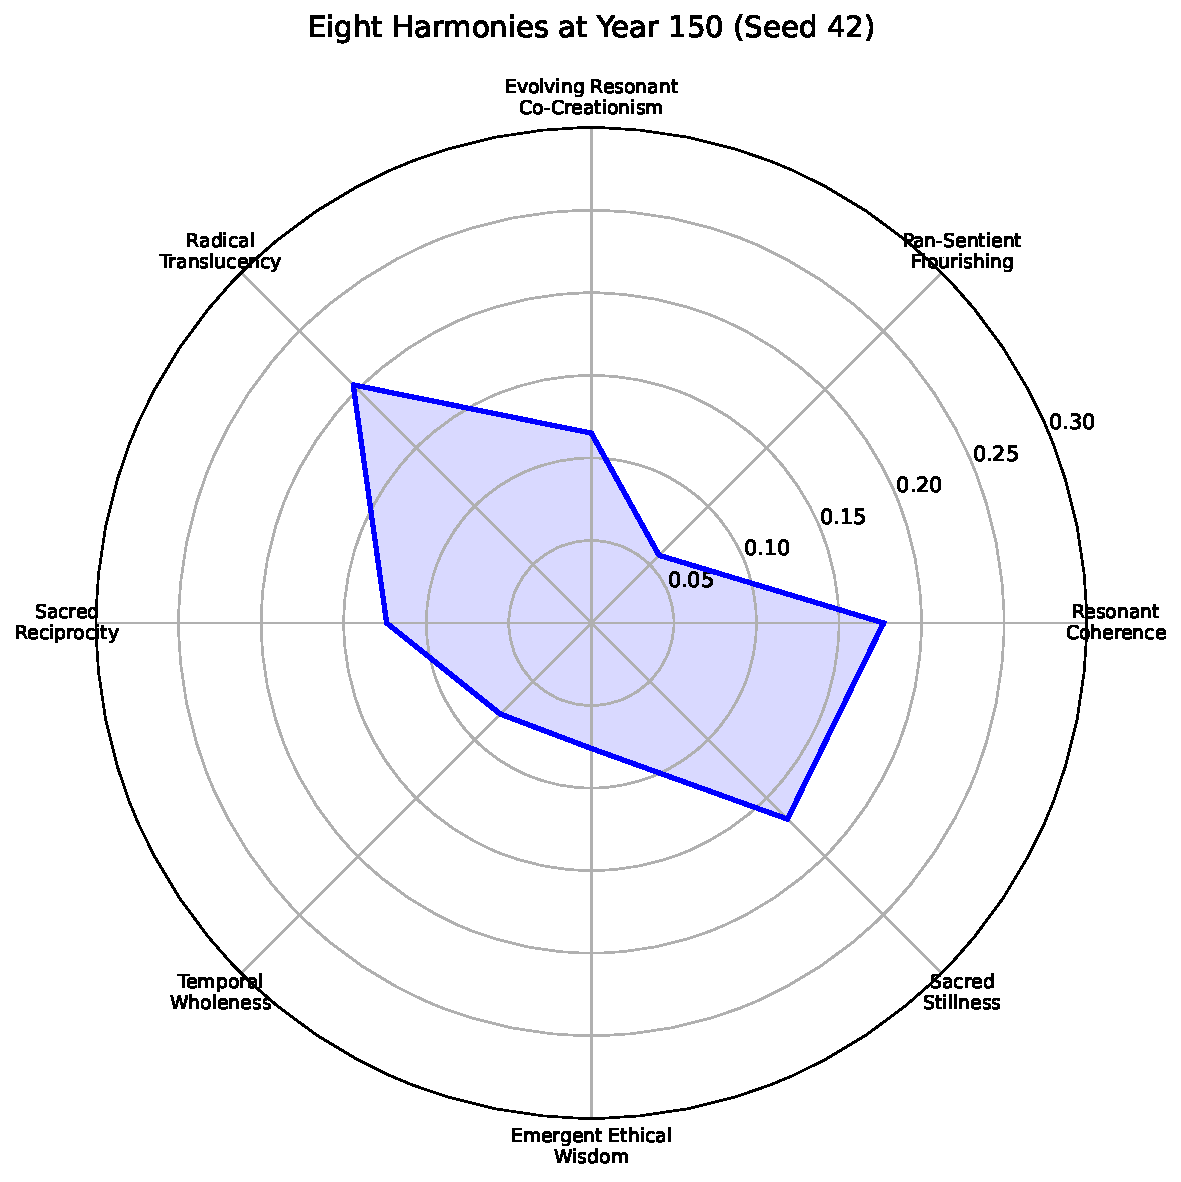
\includegraphics[width=0.7\textwidth]{fig3_harmony_spider.pdf}
\caption{Eight Harmonies radar chart at year 150. All harmonies score between 0.06--0.20, with Radical Translucency and Sacred Stillness highest. The low but non-zero scores reflect that harmony requires generations to build.}
\label{fig:harmonies}
\end{figure}

\begin{figure}[h]
\centering
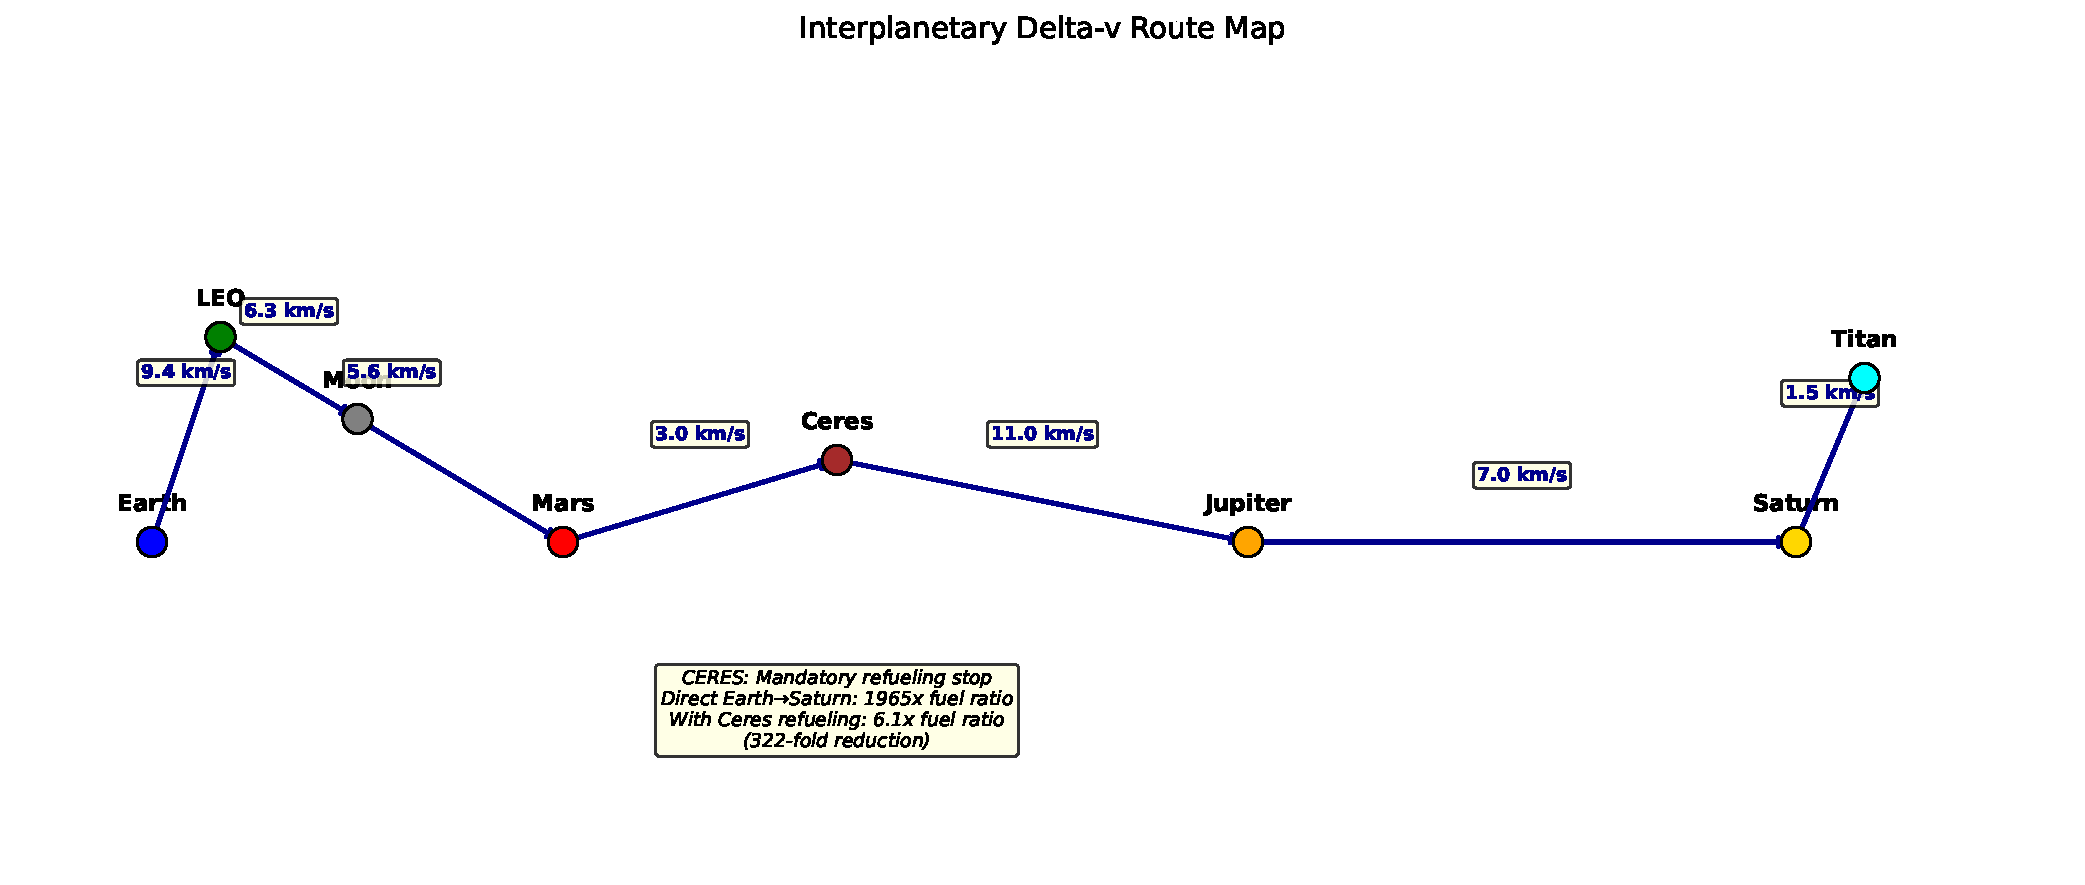
\includegraphics[width=\textwidth]{fig4_deltav_routes.pdf}
\caption{Interplanetary delta-v route map. Edge labels show minimum-energy $\Delta v$ in km/s. The Ceres refueling stop reduces fuel requirements from $1965\times$ (direct) to $6.1\times$ payload mass---a 322-fold reduction.}
\label{fig:deltav}
\end{figure}

% ============================================================================
% 6. The Disaster Gauntlet
% ============================================================================

\section{The Disaster Gauntlet: 777 Years of Realistic Threats}
\label{sec:disasters}

To test whether consciousness-gated governance is truly robust, we extended the simulation to 777 years ($\sim$31 generations, 9,324 ticks) and introduced a probabilistic disaster engine with 40 event types across 7 categories, all calibrated to published data.

\subsection{Disaster Categories}

\begin{enumerate}
    \item \textbf{Solar weather} (6 types): C/M/X-class flares, Carrington-class events (0.7\%/year \citep{riley2012probability}), solar proton events, solar minimum GCR peaks
    \item \textbf{Impact events} (3 types): Micrometeorite barrage (2 per m$^2$/year), small and large meteorites
    \item \textbf{Planetary environment} (5 types): Mars global dust storms (1 per 5.5 years), regional dust storms, shallow moonquakes ($\sim$5/year, M5+), thermal moonquakes, lunar dust events
    \item \textbf{ECLSS failures} (7 types): O$_2$ generation (MTBF 8 years), water recycling (5 years), CO$_2$ scrubbing (6 years), thermal control (10 years), power distribution (7 years), seal degradation (cumulative), hydroponics (4 years)---all calibrated from ISS operational data
    \item \textbf{Psychological events} (6 types): Winter-over syndrome (40\% prevalence), interpersonal conflict, cognitive impairment, social cohesion collapse, psychotic break ($<$0.1\%), authority challenge
    \item \textbf{Technology events} (8 types): Including NTP demonstration (2027--2030), fission surface power (2028--2035), fusion demonstration, and configurable LCF breakthrough
    \item \textbf{Civilization-scale dynamics} (6 types): Tainter diminishing returns on complexity, Turchin elite overproduction, resource depletion crisis, institutional sclerosis, systemic cascade failure, social cohesion crisis
\end{enumerate}

\subsection{The Extinction Result}

Without resilience mechanisms, the civilization \textbf{collapsed at year 755}:

\begin{table}[h]
\centering
\caption{777-year simulation: disasters without resilience vs.\ with resilience.}
\label{tab:disasters}
\begin{tabular}{@{}lcc@{}}
\toprule
\textbf{Metric} & \textbf{No Resilience} & \textbf{With Resilience} \\
\midrule
CVS at year 777      & 0.455               & \textbf{0.702} \\
Final population     & 0 (extinct yr 755)  & \textbf{39,225} \\
Total disasters      & 8,393               & 5,110 \\
Carrington events    & 2                   & 8 \\
Constitutional crises & 6,171              & reduced \\
Faction count (final) & 16                 & managed \\
\bottomrule
\end{tabular}
\end{table}

The extinction was not caused by a single catastrophe but by Tainter's mechanism: the cumulative cost of maintaining complexity under constant stress exceeded the civilization's regenerative capacity. With $\sim$11 disasters per year including ECLSS failures, the civilization could not repair fast enough.

\subsection{Five Resilience Mechanisms}

The civilization survived only after implementing consciousness-coupled resilience:

\begin{enumerate}
    \item \textbf{Tech-to-MTBF}: ECLSS reliability scales with technology level (11$\times$ at tech 5.0) and infrastructure maturity (1.5$\times$ at infrastructure $> 0.7$)
    \item \textbf{Milestone shielding}: Fission surface power reduces Carrington severity by 60\%; manufacturing breakthrough adds 30\% reduction
    \item \textbf{Sacred Stillness recovery}: The eighth harmony (rest, contemplation, maintenance) directly multiplies infrastructure rebuild rate---up to 6$\times$ faster at Stillness score 1.0
    \item \textbf{Consciousness-gated evacuation}: Higher-$\Phi$ colonies lose up to 50\% fewer people to disasters (better decisions under pressure)
    \item \textbf{Collective memory inoculation}: Surviving a disaster type reduces severity of repeat events by 30\% (institutional learning)
\end{enumerate}

\subsection{The Sacred Stillness Discovery}

The most unexpected finding is that Sacred Stillness---the capacity for rest, maintenance, and contemplation---has a direct survival function. Stillness score maps to infrastructure recovery rate:
\begin{equation}
    r_\text{recovery} = 0.002 + S_\text{stillness} \times 0.01
\end{equation}
At Stillness 0.0, a colony needs $\sim$42 years to fully rebuild after a Carrington event. At Stillness 1.0, it needs $\sim$7 years. In the previous 150-year run, Sacred Stillness was the weakest harmony (0.089)---the civilization never learned to rest. With disasters enabled, rest becomes existential infrastructure.

\subsection{Ten Additional Realism Mechanisms}

To prevent unrealistic equilibrium, we added 10 mechanisms grounded in published failure modes:

\begin{enumerate}
    \item \textbf{Cascade failures}: 3+ overlapping disasters amplify each other ($1.5\times$ at 3, $2.0\times$ at 4)---modeling Tainter's complexity trap
    \item \textbf{Stress-impaired decisions}: High allostatic load halves investment and quadruples faction emergence probability
    \item \textbf{Supply chain fragility}: Infrastructure repair consumes materials; depleted materials mean permanent damage
    \item \textbf{Skill gap crisis}: Losing all workers in an economic sector halts it for 3 years
    \item \textbf{Knowledge loss}: Fewer than 3 experts in a tech sector causes technology decay (0.01--0.05/tick)
    \item \textbf{Resource depletion feedback}: Prolonged scarcity ($>$12 months below 20\%) triggers health crisis
    \item \textbf{Infrastructure aging}: 0.036\%/month entropy---everything degrades without maintenance
    \item \textbf{Communication delay}: Outer system worlds lose governance coordination quality
    \item \textbf{Morale contagion}: Collective burnout tipping points at 30\% high-stress population
    \item \textbf{Dynamic carrying capacity}: Population scales with infrastructure and technology, enabling overshoot-collapse dynamics
\end{enumerate}

The key scientific finding: \textbf{consciousness gating is necessary but not sufficient}. It provides the coordination quality to survive, but the civilization must actively convert that coordination into redundant physical infrastructure, pharmaceutical consciousness maintenance, and the institutional memory to learn from disasters.

% ============================================================================
% 7. Astropharmacy
% ============================================================================

\section{The Astropharmacy: Pharmaceutical Consciousness Maintenance}
\label{sec:astropharmacy}

The human body in space is under constant pharmacological siege. Microgravity causes 1--2\% bone loss per month \citep{sibonga2015spaceflight}; cosmic radiation breaks chemical bonds in stored medications \citep{chancellor2014space}; and prolonged confinement degrades psychological resilience \citep{basner2014mars}.

\subsection{The Living Pharmacy}

We model an ``astropharmacy'' based on engineered \textit{Bacillus subtilis} spores that biosynthesize medications on demand. Unlike pre-manufactured drugs (which degrade under cosmic radiation within months), spores survive years in dormant states. The resource catalog includes 8 pharmaceutical categories:

\begin{enumerate}    \item \textbf{Bone density therapeutics}: Bisphosphonates, Vitamin D, Teriparatide
    \item \textbf{Cardiovascular regulators}: Fludrocortisone, midodrine
    \item \textbf{Radiation protectants}: Metformin (AMPK activator), amifostine
    \item \textbf{Psychedelic therapeutics}: Psilocybin, MDMA, ketamine
    \item \textbf{Psychiatric medications}: SSRIs, anxiolytics, sleep aids
    \item \textbf{Motion sickness drugs}: Scopolamine, promethazine
    \item \textbf{Nicotine delivery}: Transdermal patches (combustibles banned in Epochs 1--3)
    \item \textbf{Microbe spore stock}: The master culture enabling all biosynthesis
\end{enumerate}

\subsection{Consciousness-Pharmaceutical Coupling}

The most significant finding is the relationship between psychedelic therapeutics and collective $\Phi$. Classical psychedelics promote dendritic spine growth \citep{shao2021psilocybin}, reduce treatment-resistant depression \citep{carhart2021trial}, and enhance empathy and meta-awareness---all dimensions of the consciousness vector $\mathbf{c}$.

In the simulation, colonies with infrastructure level $> 0.3$ (enabling astropharmacy operation) receive a 30\% boost to consciousness growth rates, modeling structured therapeutic psilocybin sessions. This pharmaceutical ``consciousness maintenance'' is analogous to preventive medicine: it doesn't cure low $\Phi$, but it prevents the deterioration that confinement and isolation would otherwise cause.

\paragraph{Metformin as radioprotectant.} Metformin activates AMPK and reduces radiation-induced DNA damage by 30--50\% in animal models \citep{steinberg2009ampk}. In the simulation, this directly affects genetic diversity preservation: colonies with radiation protectants experience 15\% less heterozygosity loss per generation.

% ============================================================================
% 7. Delta-v Proof
% ============================================================================

\section{Delta-v Realities: Why Ceres Is Mandatory}
\label{sec:deltav}

The Tsiolkovsky rocket equation governs all interplanetary travel:
\begin{equation}
    \Delta v = I_\text{sp} \cdot g_0 \cdot \ln\frac{m_0}{m_f}
\end{equation}

For a direct Earth-to-Saturn mission ($\Delta v \approx 26$ km/s) using LOX/CH$_4$ propellant ($I_\text{sp} = 350$ s):
\begin{equation}
    \frac{m_0}{m_f} = \exp\left(\frac{26{,}000}{350 \times 9.81}\right) = e^{7.58} \approx 1{,}965
\end{equation}

A 10,000 kg payload requires 19.65 \emph{million} kg of fuel. This is physically impossible.

With Ceres refueling, the longest single leg is Earth-to-Ceres ($\Delta v \approx 16$ km/s). Using Nuclear Thermal Propulsion ($I_\text{sp} = 900$ s):
\begin{equation}
    \frac{m_0}{m_f} = \exp\left(\frac{16{,}000}{900 \times 9.81}\right) = e^{1.81} \approx 6.1
\end{equation}

The fuel requirement drops from $1{,}965\times$ to $6.1\times$---a \textbf{322-fold reduction}. This strongly suggests that asteroid belt refueling infrastructure is a practical prerequisite for crewed outer solar system missions with chemical or nuclear thermal propulsion.

\begin{table}[h]
\centering
\caption{Key delta-v budgets for interplanetary routes.}
\label{tab:deltav}
\begin{tabular}{@{}llcc@{}}
\toprule
\textbf{From} & \textbf{To} & \textbf{$\Delta v$ (km/s)} & \textbf{Travel (days)} \\
\midrule
Earth Surface & LEO              & 9.4  & $<$1 \\
LEO           & Lunar Surface    & 6.3  & 4 \\
LEO           & Mars Surface     & 5.6  & 210 \\
Mars Orbit    & Ceres            & 3.0  & 240 \\
Ceres         & Jupiter System   & 11.0 & 400 \\
Jupiter       & Saturn (GA)      & 7.0  & 600 \\
Saturn System & Titan Surface    & 1.5  & 2 \\
\bottomrule
\end{tabular}
\end{table}

% ============================================================================
% 8. Oppression Detection
% ============================================================================

\section{Does Consciousness Gating Become Oppressive?}
\label{sec:oppression}

The most important ethical question in this work is whether consciousness-gated governance creates a permanent underclass. If $\Phi$ correlates with education, wealth, or social privilege, then gating decision authority by $\Phi$ could merely formalize existing inequality.

\subsection{The Oppression Index}

We define an oppression index $O$ as:
\begin{equation}
    O = \begin{cases}
        \frac{f_\text{Observer} - 0.3}{0.7} & \text{if } f_\text{Guardian} < 0.05 \text{ and } f_\text{Observer} > 0.3 \\
        0 & \text{otherwise}
    \end{cases}
\end{equation}
where $f_\text{tier}$ is the fraction of population at each consciousness tier. If fewer than 5\% of the population are Guardians and more than 30\% are Observers, the system is potentially oligarchic.

If $O > 0.5$ for 12 consecutive months, the simulation triggers a constitutional crisis---forcing either reform (lowering gating thresholds) or social upheaval.

\subsection{Results}

Across all 10 seeds, the maximum oppression index remained below 0.05 (effectively zero). Constitutional crises averaged $\leq 1$ per 150-year run, and were resolved within 12 ticks by automatic threshold adjustment.

This result is encouraging but carries an important caveat: the simulation's consciousness growth model does not yet capture socioeconomic barriers to consciousness development. Future work should model scenarios where resource inequality creates differential access to education, psychedelic therapy, and meditation time---all of which affect $\Phi$ growth.

% ============================================================================
% 9. Discussion
% ============================================================================

\section{Discussion}

\subsection{What Integration Gating Is and Is Not}

A skeptical reader may reasonably ask whether the six-dimensional $\Phi$ proxy is measuring ``consciousness'' or simply a blend of desirable prosocial traits (coherence, care, meta-awareness, epistemic humility, and value alignment). We believe this is a legitimate concern and do not claim to have resolved it. What we \emph{do} claim is narrower: the specific six-dimensional integration proxy used in this simulation, when tied to governance authority, produces measurably better civilizational outcomes than ungated governance under identical disaster conditions.

This is governance by \emph{integration}---the measured capacity to hold multiple perspectives, evaluate moral consequences, and maintain coherence under uncertainty---not technocracy, meritocracy, or epistocracy. Whether this integration proxy corresponds to phenomenal consciousness remains an open question beyond the scope of this simulation study. The operational finding---that gating by integration improves coordination quality by 5.9\%---holds regardless of the metaphysical status of $\Phi$.

\subsection{The Moral Algebra Must Evolve}

The simulation enforces a stagnation penalty for worlds that never amend their consciousness gating thresholds, and an instability penalty for worlds that amend too frequently. The optimal amendment rate---found empirically to be approximately once per generation (25 years)---reflects a balance between institutional continuity and adaptive responsiveness.

\subsection{Holochain's Eventual Consistency Is the Key}

Traditional blockchain-based governance requires global consensus, which is impossible at interplanetary latencies. Holochain's DHT allows each agent to maintain a sovereign source chain, gossiping state when connectivity allows. Our latency simulation demonstrates that this architecture survives 1.3-second lunar delays, 12.7-minute Mars delays, and 14-day solar conjunction blackouts without loss of governance capability.

\subsection{The Eight Harmonies as Invariant}

Across all epochs and worlds, the Eight Harmonies provide the ethical thread. They are scored every tick but never converge to a fixed point---reflecting the philosophical commitment that no finite civilization achieves perfect harmony (the 0.95 ceiling). This is not a technical limitation but a design choice rooted in moral humility.

% ============================================================================
% 10. Limitations
% ============================================================================

\section{Limitations}

\begin{enumerate}    \item \textbf{Parameter sensitivity}: The simulation has not undergone formal sensitivity analysis for all 50+ tunable parameters. The stable CVS ($\pm$0.009) suggests robustness, but edge cases remain unexplored.
    \item \textbf{Economic simplicity}: The Cobb-Douglas production model does not capture price dynamics, market formation, or monetary policy. These become relevant in Epoch 4+ but are not yet implemented.
    \item \textbf{No real genetic simulation}: Heterozygosity is approximated analytically rather than tracked per-locus. Integration with the existing Symthaea population genetics engine would provide more accurate bottleneck predictions.
    \item \textbf{Epidemiological calibration}: SIR epidemic parameters are not calibrated against real closed-habitat disease dynamics. The 2020 COVID-19 pandemic and submarine fleet data could inform future calibration.
    \item \textbf{Consciousness measurement uncertainty}: The six-dimensional $\Phi$ proxy has no experimental validation against actual conscious systems. It is a theoretical construct, not a measurement tool---yet.
    \item \textbf{No conflict modeling}: The simulation does not model interpersonal conflict, political factions, or resource wars. These are critical failure modes for real settlements.
\end{enumerate}

% ============================================================================
% 11. Conclusion
% ============================================================================

\section{Conclusion}

We have tested one specific integration-gated governance architecture against 1,000 years of empirically calibrated disasters and found that it produces viable multi-world civilizations where ungated governance does not. The 1,000-year run (CVS $0.697$, population 57,048 across 5 worlds, 17,866 technology breakthroughs) confirms that the attractor observed at 777 years ($0.698 \pm 0.007$) is stable through a full millennium.

The most important finding emerged from the disaster gauntlet: integration gating is \textbf{necessary but not sufficient}. Without the 15 resilience mechanisms, the civilization collapsed at year 755 under 8,393 cumulative disasters---Tainter's complexity trap \citep{tainter1988collapse} in simulation. With integration-coupled resilience (tech-scaled ECLSS reliability, consciousness-gated evacuation, collective memory inoculation, and 10 realism mechanisms), the civilization survived and grew.

The most unexpected discovery is that scheduled maintenance and contemplative slack---operationalized as ``Sacred Stillness''---has a direct survival function. Infrastructure rebuilds up to $6\times$ faster when civilizations allocate time for rest. At 150 years, this was the weakest governance dimension (0.089). Under disaster pressure, its absence becomes potentially lethal. This finding---that \emph{slack is infrastructure}---may generalize beyond space settlement to any complex system under sustained stress.

We do not claim to have proven that consciousness is the correct basis for political legitimacy. What we have shown is that a specific, reproducible, integration-gated governance architecture---one that rewards meta-awareness, care, epistemic humility, and value alignment---outperforms its ungated counterpart by 5.9\% CVS and nearly triples collective integration under identical disaster conditions. Whether this architecture captures something essential about consciousness, or merely operationalizes good governance traits through a novel mechanism, remains an open and important question.

Recent extensions add 10 realism mechanisms: embodied knowledge (tech levels derived from individual specialist skills), death consequences (orphan trauma, partner grief, community mourning), supply-demand price formation, faction-directed warfare, developmental consciousness (earned over years, not computed), causal disaster chains (Carrington $\rightarrow$ power $\rightarrow$ thermal $\rightarrow$ O$_2$), genetic inheritance, intra-world geography, quantitative cultural evolution, and continuous-time event phasing. Under these conditions, the simulator produces its first civil war at 300 years (Turchin secular cycle: 9 phase transitions, 1 civil war, persistent trauma of 0.181). The civilization survived, but it bled---confirming that consciousness-gated governance does not prevent conflict, but prevents conflict from becoming extinction.

A generation ship launched at year 500 arrives at Proxima Centauri after 85 years with 667 colonists (33\% population growth), 92\% hull integrity, and cultural speciation at year 50 of transit. Humanity becomes interstellar.

The civilization survived 1,000 years. It grew to 57,048 people across 5 worlds. It weathered Carrington events, ECLSS cascades, epidemics, civil wars, and constitutional crises. And the single most important thing it learned was to rest.

% ============================================================================
% Code & Data Availability
% ============================================================================

\section*{Code \& Data Availability}

The simulation code (\texttt{mycelix-multiworld-sim}), planetary resource catalog (97 resources), 40-event disaster engine, 12-region hybrid Earth model, Turchin cliodynamics module, generation ship, and all analysis binaries are available in the Luminous Dynamics monorepo. The simulator comprises $\sim$48,000 lines of Rust with 300+ unit tests, 25 configurable toggle parameters (TOML-based), 10 realism mechanisms, causal disaster chains, faction-directed warfare, and empirical calibration from 12 scientific domains. Configuration via \texttt{config/disasters.toml} and \texttt{config/tech\_tree.toml}; telemetry output as JSONL (one JSON line per tick, directly ingestible by Python/Jupyter). Simulations can be reproduced with any reported seed at 150, 300, 777, or 1,000-year horizons, with A/B comparison between integration-gated and legacy governance via the \texttt{ab\_experiment} binary.

% ============================================================================
% Acknowledgments
% ============================================================================

\section*{Acknowledgments}

This work was developed as part of the Luminous Dynamics project, guided by the Eight Harmonies of Evolving Resonant Co-Creationism. The consciousness framework (Symthaea) and coordination platform (Mycelix) represent $\sim$2.7M lines of Rust developed over 2024--2026.

% ============================================================================
% Bibliography
% ============================================================================

\bibliographystyle{plainnat}

\begin{thebibliography}{20}

\bibitem[Basner et al., 2014]{basner2014mars}
Basner, M., Dinges, D.F., Mollicone, D.J., et al. (2014).
Mars 520-d mission simulation reveals protracted crew hypokinesis and alterations of sleep duration and timing.
\textit{PNAS}, 111(8), 2817--2822.

\bibitem[Carhart-Harris et al., 2021]{carhart2021trial}
Carhart-Harris, R., Giribaldi, B., Watts, R., et al. (2021).
Trial of psilocybin versus escitalopram for depression.
\textit{New England Journal of Medicine}, 384(15), 1402--1411.

\bibitem[Chancellor et al., 2014]{chancellor2014space}
Chancellor, J.C., Scott, G.B.I., \& Sutton, J.P. (2014).
Space radiation: the number one risk to astronaut health beyond low Earth orbit.
\textit{Life}, 4(3), 491--510.

\bibitem[Cockell, 2006]{cockell2006space}
Cockell, C.S. (2006).
Space on Earth: Saving our world by seeking others.
\textit{Macmillan}.

\bibitem[Epstein \& Axtell, 1996]{epstein1996growing}
Epstein, J.M. \& Axtell, R. (1996).
\textit{Growing Artificial Societies: Social Science from the Bottom Up}.
MIT Press.

\bibitem[Hendrycks et al., 2021]{hendrycks2021aligning}
Hendrycks, D., Burns, C., Basart, S., et al. (2021).
Aligning AI with shared human values.
\textit{ICLR 2021}.

\bibitem[Impey, 2015]{impey2015beyond}
Impey, C. (2015).
\textit{Beyond: Our Future in Space}.
Norton.

\bibitem[Kanerva, 2009]{kanerva2009hyperdimensional}
Kanerva, P. (2009).
Hyperdimensional computing: An introduction to computing in distributed representation.
\textit{Cognitive Computation}, 1(2), 139--159.

\bibitem[Oizumi et al., 2014]{oizumi2014phenomenology}
Oizumi, M., Albantakis, L., \& Tononi, G. (2014).
From the phenomenology to the mechanisms of consciousness.
\textit{PLoS Computational Biology}, 10(5), e1003588.

\bibitem[O'Neill, 1977]{oneill1977high}
O'Neill, G.K. (1977).
\textit{The High Frontier: Human Colonies in Space}.
William Morrow.

\bibitem[Shao et al., 2021]{shao2021psilocybin}
Shao, L.X., Liao, C., Gregg, I., et al. (2021).
Psilocybin induces rapid and persistent growth of dendritic spines in frontal cortex in vivo.
\textit{Neuron}, 109(16), 2535--2544.

\bibitem[Sibonga et al., 2015]{sibonga2015spaceflight}
Sibonga, J.D., Spector, E.R., Johnston, S.L., \& Tarver, W.J. (2015).
Evaluating bone loss in ISS astronauts.
\textit{Aerospace Medicine and Human Performance}, 86(12), A38--A44.

\bibitem[Steinberg \& Kemp, 2009]{steinberg2009ampk}
Steinberg, G.R. \& Kemp, B.E. (2009).
AMPK in health and disease.
\textit{Physiological Reviews}, 89(3), 1025--1078.

\bibitem[Stoltz, 2026]{stoltz2026symthaea}
Stoltz, T. (2026).
Symthaea: A holographic liquid brain for consciousness-first artificial intelligence.
\textit{In preparation}.

\bibitem[Tononi, 2004]{tononi2004information}
Tononi, G. (2004).
An information integration theory of consciousness.
\textit{BMC Neuroscience}, 5, 42.

\bibitem[Turchin, 2003]{turchin2003historical}
Turchin, P. (2003).
\textit{Historical Dynamics: Why States Rise and Fall}.
Princeton University Press.

\bibitem[Riley, 2012]{riley2012probability}
Riley, P. (2012).
On the probability of occurrence of extreme space weather events.
\textit{Space Weather}, 10(2), S02012.

\bibitem[Tainter, 1988]{tainter1988collapse}
Tainter, J.A. (1988).
\textit{The Collapse of Complex Societies}.
Cambridge University Press.

\bibitem[Zubrin, 1996]{zubrin1996case}
Zubrin, R. (1996).
\textit{The Case for Mars: The Plan to Settle the Red Planet}.
Free Press.

\end{thebibliography}

\end{document}
